\documentclass[11pt]{article}
\usepackage[margin=1in]{geometry}
\usepackage{graphicx}
\usepackage{subcaption}
\title{GPU accelerated ray tracing}
\author{William Zhang}
\date{\today}

\begin{document}
\maketitle
\section{Background}
Ray tracing is a rendering technique designed to more closely model the physical characteristics
of light compared to techniques such as rasterization while also being less computationally
expensive than techniques such as global illumination. Conceptually, ray tracing traces rays of light
backwards from the eye of the viewer to all objects in a scene. By using some function to approximate
the scattering of light on incidence with an object, ray tracing provides realistic visuals for a 
variety of materials.

As each pixel is independent from another, ray tracing is easily parallelizable by dividing the 
pixels among parallel workers. In this project, I parallelize ray tracing by designating a
GPU thread per pixel. My hypothesis was that this would achieve dramatic speedup compared to a
serial implementation and would strongly scale due to the limited need of communication as well
as synchronization. I also hypothesized that ray tracing would be highly sensitive to the kernel
parameters, as more distant pixels tend to have significantly more different distributions in 
the amount of rays broadcast and collisions performed.

\section{Design}
\subsection{Serial Implementation}
My serial raytracer implements support for secondary rays such as reflection and refraction and
shadow and distance attenuation of light intensity through objects. For each pixel, a ray is propagated
throughout the scene and checked for collisions with any objects. On collision, a \textit{shadow ray} is 
spawned towards every light source to calculate the degree in which the object is obscured from a nearby
light source. The \textit{secondary} reflection and refraction rays are spawned recursively should the collided object be 
transluscent or reflective. Contributions are all additive, but clamped to be in the range $[0.0, 1.0]$.
The final values are scaled to 255 to determine the value for each color channel. I support all 4 color
channels of the RGBA system, albeit the alpha channel is rarely set to a value different than 1.

Each object is represented as a collection of triangles that form a \textit{trimesh}. I chose triangles as the only
primitive to implement as every other primitive can be represented with triangles, including round objects such
as spheres through careful manipulation of triangle normal vectors. Each triangle component of an object is free
to have unique material properties, supporting complex object types. Objects can be duplicated with little cost by 
providing transformations such as translation and rotation to them. I also assume all objects have no gaps, and that
there are no objects within other objects.

In addition, I implement a bounding volume heirarchy (BVH) tree to prune a large portion of objects to perform collision
detection. A BVH tree is a binary tree that generates bounding boxes for nearby objects as a collective such that
if a ray misses the encompassing bounding box, it is guaranteed to miss all objects within it. Each leaf node of
the binary tree represents a specific scene object, while each inner node consists of a bounding box that encompasses
all its descendants. I constructed BVH trees by first sorting the objects by a space filling curve and then 
merging bottom-up between adjacent nodes. BVH iteration is performed recursively.

\subsection{Parallel Implementation}
My parallel raytracer implements the same features as the serial one. To support secondary rays, all recursion is
converted to an iterative counterpart, where state is stored on a stack and transitions between states are coded explicitly.
Likewise, BVH iteration was performed iteratively as well. Iteration must be used as although modern GPUs support recursion,
compilers cannot statically determine parameters such as the stack size. Stacks also reside in local memory, which
has high latency as it resides off chip.

In addition, my implementation uses the texture cache to store triangle vertices and normals. Although most GPUs have a designated
vertex cache, CUDA does not expose it. The texture cache is optimized for constant memory and the local coordinates of the triangle 
vertices never change irregardless of transformations, making it the next best choice.

Parallelization of raycasting simply involved broadcasting a ray per pixel as explained previously. BVH generation was parallelized
by using the Thrust library to sort by morton code, then doing a reduction per level until the tree was constructed.

\section{Results}

\begin{figure}
    \centering
    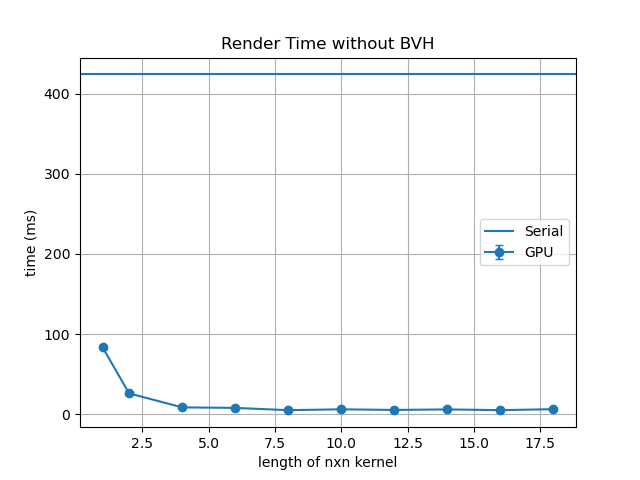
\includegraphics[scale=.6]{world1b1.png}
    \caption{Large speedups immediately apparent prior to BVH integration. Error bars indicate standard deviation.}
    \label{fig:no_bvh}
\end{figure}

\begin{figure}
    \centering
    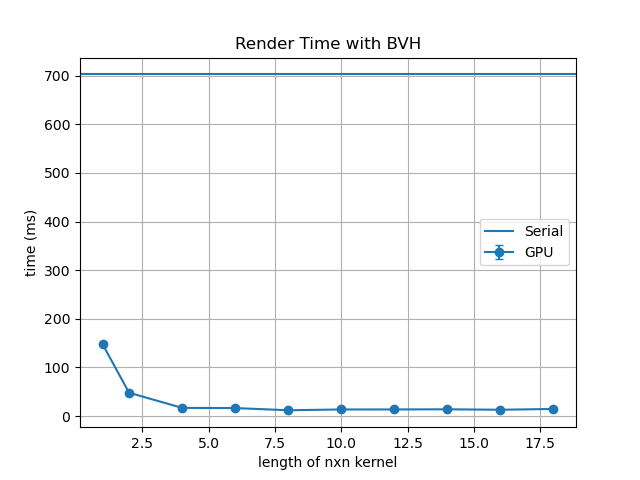
\includegraphics[scale=.6]{world8b8.png}
    \caption{Similar speedups with BVH integration. Error bars indicate standard deviation.}
    \label{figure:bvh}
\end{figure}

\begin{figure}
    \centering
    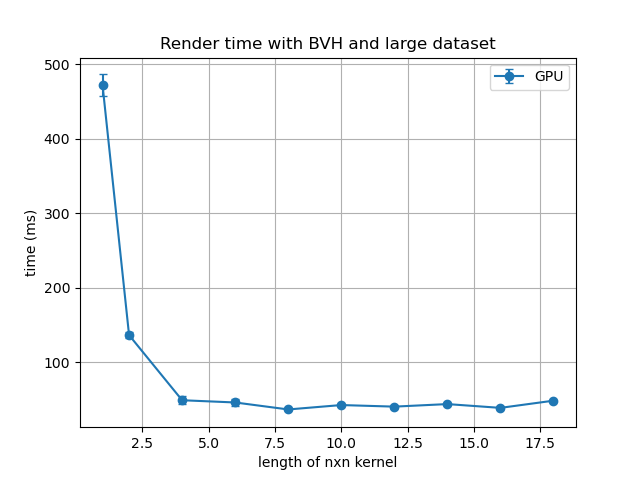
\includegraphics[scale=.6]{world16b16.png}
    \caption{Larger dataset with BVH integration. Error bars indicate standard deviation.}
    \label{figure:large}
\end{figure}

GPU accelerating the process demonstrated remarkable speedup. As shown in Figure~\ref{fig:no_bvh}, even with a one by one block, a four-time speedup was
observed. This initially surprised me, but as the GPU can schedule each one by one block to a different streaming multiprocessor, parallelism can still be
achieved. I was also surprised by the result since I was initially under the impression that GPU cores were significantly slower than their CPU counterparts
to gain any speedup with a low number of threads. The asymptotic decrease does confirm to me of strong scaling confirming my first hypothesis. However, it does
not appear that the kernel dimension was very important, as increasing the block size at a certain part did not cost anything. BVH integration surprisingly closed 
the gap a little, but the same trends are seen (Figure~\ref{figure:bvh}). 

A concern from the results I had was how quickly the graphs plateaued in Figure~\ref{figure:large}. With raytracing being inherently parallel with few synchronization, I expected the 
parallel component in Amdahl's law of strong scaling to vastly overtake the serial component. I thought the bottleneck to further parallelization could involve
memory copying to and from the device, but the results of Figure~\ref{fig:no_bvh} suggest otherwise. The footprint of copying would have affected all runs including
those that terminated in under 5 ms, suggesting copying is not the source. Through profiling on nvprof, despite having a high L1 cache hit rate, memory bottlenecks 
during execution seemed to dominate.

Further analysis in the profiler suggested that my execution model may also be flawed. As of now, after spawning a few kernels for BVH construction, only one kernel
is spawned for the entire ray tracing process. Perhaps determining a way to rewrite it such that multiple kernels run asynchronously would provide higher speedup.
As of now, only roughly 50\% of the GPU is being utilized according to nvprof due to heavyweight kernels requiring too many registers to spawn more threads. By breaking
the kernel apart, potentially I could decrease the memory footprint of each kernel and increase utilization.

\section{Limitations and Future Work}
Shared memory was not utilized at all during the implementation of this project. Due to the large size of metadata associated with collisions
and objects, at this time, I could not determine when it would be useful to use. To reach desired speeds, it is imperative that the ray tracer
eventually exploits it in the future. In addition, more complex features have not yet been implemented, such as caustics, constructive solid geometry,
and texture mapping.

\end{document}